%%\documentclass[a4paper,11pt]{article}
\documentclass[11pt]{article}

\usepackage[left=2.5cm, right=2cm, top=1.5cm, bottom=3cm]{geometry}
\usepackage[utf8]{inputenc}
\usepackage[T1]{fontenc}
\usepackage{titlesec}
\usepackage{enumitem}
\usepackage{graphicx}
\usepackage{amsmath}
\usepackage{amsfonts}
\usepackage{amssymb}
\usepackage{parskip}
\usepackage{float}
\usepackage{setspace}
\usepackage{fancyhdr}

\pagestyle{fancy}
\fancyhf{}
\setlength{\headheight}{65pt}
\setlength{\headsep}{24pt}
\fancyhead[L]{
\includegraphics[height=1.5cm]{picture/logo.pdf}}
\fancyhead[R]{\textbf{Ingeniería de Software 2026}}
\renewcommand{\headrulewidth}{0.4pt}
\fancyfoot[C]{\thepage}
\setlength{\footskip}{14pt}

\setstretch{1.12}
\setlength{\parskip}{0.65em}
\setlist[itemize]{leftmargin=1.35cm, itemsep=0.45em, topsep=0.35em}
\setlist[enumerate]{leftmargin=1.35cm, itemsep=0.45em, topsep=0.35em}

\titleformat{\section}{\normalfont\Large\bfseries}{\thesection}{1em}{}
\titleformat{\subsection}{\normalfont\large\bfseries}{\thesubsection}{1em}{}

\title{Informe del Proyecto}

\begin{document}

\renewcommand{\thesection}{\Roman{section}}
\begin{center}
    \textbf{\underline{\normalsize APE 1}}
\end{center}

\section{PORTADA}

\begin{tabbing}
    \textbf{Tema:}\hspace{1cm} \= Ecualizador Modular para Procesamiento de Imágenes \\[0.25em]
    \textbf{Carrera:}\hspace{1cm} \= Ingeniería de Software \\[0.25em]
    \textbf{Unidad de Organización Curricular:} \hspace{1cm} \= PROFESIONAL \\[0.25em]
    \textbf{Nivel y Paralelo:} \> Séptimo semestre A \\[0.25em]
    \textbf{Alumnos participantes:} \> Paul Velastegui \\
    \> David Manjarres \\[0.25em]
    \textbf{Asignatura:} \> Gestión de Proyectos \\[0.25em]
    \textbf{Docente:} \> Ing. Rubén Nogales, Mg.
\end{tabbing}

\section{INFORME DE GUÍA PRÁCTICA}
\renewcommand{\thesection}{\arabic{section}}

\subsection{Objetivos}
\textbf{General:}
\begin{itemize}
    \item Aplicar un flujo de preprocesamiento de imágenes bajo arquitectura MVVM que permita la mejora del contraste mediante normalización min-max por canal, la conversión a escala de grises, la compresión espacial por bloques y la segmentación binaria por umbralización, evaluando el sistema con imágenes de alta complejidad espectral.
\end{itemize}

\textbf{Específicos:}
\begin{itemize}
    \item Analizar la distribución de intensidades de la imagen original mediante histogramas por canal R, G y B, antes y después de aplicar la normalización min-max, para evidenciar la expansión del contraste.
    \item Implementar la normalización min-max de forma independiente sobre cada canal RGB usando NumPy y OpenCV, reconstruyendo la imagen base a partir de los tres canales normalizados.
    \item Obtener la imagen comprimida en escala de grises mediante promediado por bloques de $N \times N$ y su versión binarizada, observando el efecto de los controles de tamaño de bloque y umbral sobre el resultado final.
\end{itemize}

\subsection{Modalidad}
\begin{tabbing}
    \hspace{1cm} \= Presencial.
\end{tabbing}

\subsection{Tiempo de duración}
\begin{tabbing}
    \hspace{1cm} \= \textbf{Presenciales:} \= 8 \\
    \hspace{1cm} \= \textbf{No presenciales:} \= 0
\end{tabbing}

\subsection{Instrucciones}
\begin{enumerate}
    \item Seleccionar una imagen de entrada para realizar el procesamiento.
    \item Normalizar la imagen y observar los cambios generados en su representación visual.
    \item Visualizar la imagen desde sus canales de color para comparar la información presente en cada uno.
    \item Comprimir la imagen en escala de grises mediante bloques de reducción.
    \item Aplicar binarización por umbral para obtener una imagen compuesta únicamente por valores claros y oscuros.
\end{enumerate}

\subsection{Listado de equipos, materiales y recursos}
Listado de equipos y materiales generales empleados en la guía práctica:
\begin{itemize}
    \item Computador.
    \item Imagen de prueba de alta complejidad espectral (región de formación estelar W51).
    \item Entorno de desarrollo Python 3 con PySide6, OpenCV y NumPy.
    \item Internet.
    \item Material disponible en el aula virtual de la asignatura.
    \item Herramientas que permitan generar documentos en formato PDF.
\end{itemize}

\textbf{TAC (Tecnologías para el Aprendizaje y Conocimiento) empleados en la guía práctica:}

$\square$ Plataformas educativas \\
$\square$ Simuladores y laboratorios virtuales \\
$\blacksquare$ Aplicaciones educativas \\
$\square$ Recursos audiovisuales \\
$\square$ Gamificación \\
$\blacksquare$ Inteligencia Artificial \\
Otros (Especifique): \underline{\hspace{5cm}}

\subsection{Actividades por desarrollar}
\begin{enumerate}
    \item Cargar la imagen de la región W51 y generar los histogramas originales por canal.
    \item Aplicar la normalización por canal y generar los histogramas normalizados.
    \item Obtener la imagen en escala de grises, comprimirla por bloques y aplicar la binarización por umbral.
    \item Comparar la imagen original, la normalizada, la comprimida en escala de grises y la binarizada.
\end{enumerate}

\subsection{Material y Caso de Estudio}

En esta sección se presenta la imagen seleccionada como caso de estudio, justificando su elección en función de su complejidad espectral y la correspondencia con los algoritmos implementados en la herramienta.

\subsubsection{Región de formación estelar W51 (James Webb Space Telescope, 2025)}

Esta es una de las imágenes más recientes y de mayor resolución obtenidas en el estudio de regiones de formación estelar en nuestra galaxia. Fue capturada por el Telescopio Espacial James Webb (JWST) por investigadores de la Universidad de Florida, con crédito oficial a NASA, ESA, CSA y el equipo Yoo \& Ginsburg (UF), con procesamiento de imágenes por A.~Pagan (STScI) \cite{jwst_w51}.

\textbf{Por qué usarla:} Al ser capturada en infrarrojo cercano (NIRCam) y medio (MIRI), posee una claridad y resolución sin precedentes. El JWST puede detectar luz infrarroja que atraviesa las nubes de polvo que bloquean la luz visible ordinaria, permitiendo observar directamente estrellas jóvenes aún envueltas en las nubes de polvo de las que nacieron \cite{jwst_w51}.

\textbf{Impacto en la aplicación:} Las imágenes muestran nubes de gas brillantes iluminadas por estrellas masivas, junto con burbujas de gas ionizado, filamentos oscuros de polvo y chorros de material expulsados por estrellas jóvenes. El procesamiento de normalización \textit{min-max} que se detalla en este informe es ideal para rescatar información en zonas de baja intensidad (estrellas ``escondidas'' detrás del gas más caliente) y revelar estructuras que en la imagen original se presentan con contraste reducido. Este análisis constituye un caso de uso real de las capacidades de la herramienta para rescatar información espectral y espacial subyacente.

\begin{figure}[H]
    \centering
    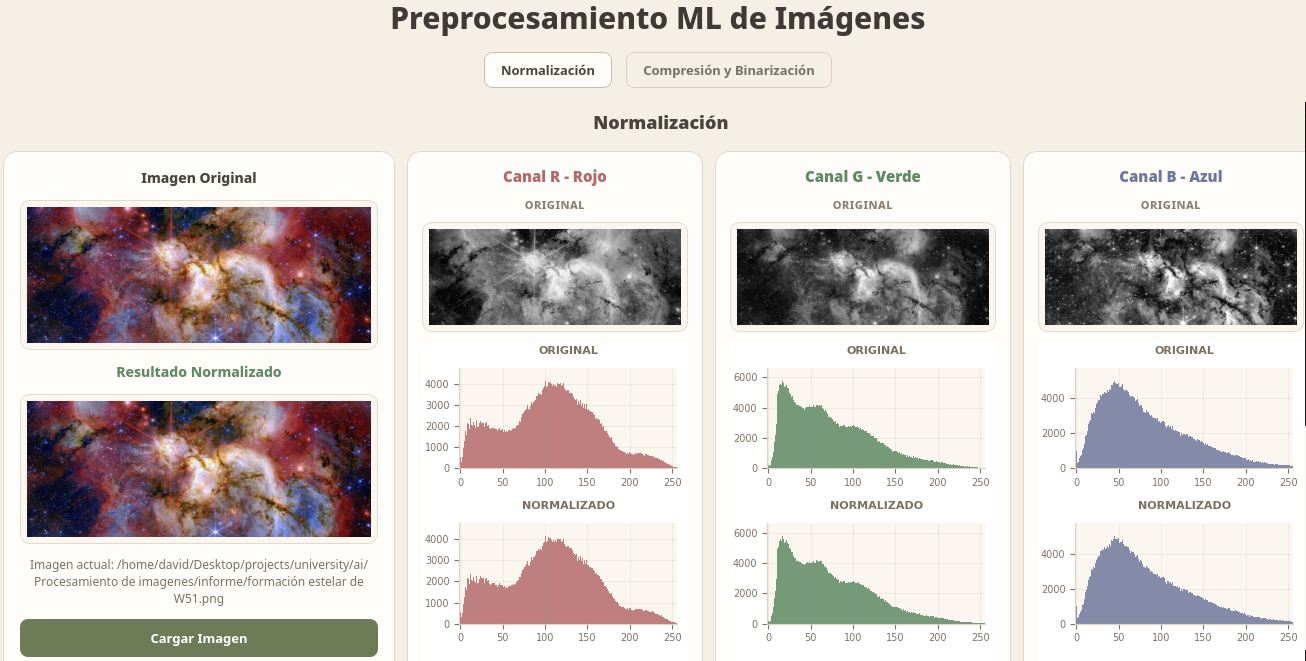
\includegraphics[width=0.92\textwidth]{img/app_interfaz_w51.png} % REEMPLAZAR: captura de la app con W51 cargada (pantalla de Normalización)
    \caption{Interfaz de la herramienta con la imagen de W51 cargada, mostrando la página de Normalización con los cuatro paneles: imagen original, canal R, canal G y canal B.}
    \label{fig:app_interfaz}
\end{figure}

\begin{figure}[H]
    \centering
    \includegraphics[width=0.82\textwidth]{"formación estelar de W51.png"}
    \caption{Región de formación estelar W51 capturada por el JWST. Crédito: NASA, ESA, CSA, Yoo \& Ginsburg (UF). Procesamiento: A.~Pagan (STScI) \cite{jwst_w51}.}
    \label{fig:w51}
\end{figure}

\subsection{Resultados obtenidos}

En esta sección se documenta el procedimiento aplicado sobre la imagen de la región estelar W51. Se parte de la imagen original, se analizan sus histogramas por canal, se aplica la normalización, se obtiene la imagen normalizada junto con su versión en escala de grises y binaria, y finalmente se comparan los resultados.

\subsubsection{Imagen original utilizada}

La imagen empleada corresponde a la región de formación estelar W51, obtenida por el JWST en el infrarrojo cercano y medio. Esta imagen constituye el punto de partida del procesamiento. Su características más relevante para los fines de esta práctica es que presenta amplias zonas de alto brillo (nubes de gas ionizado) junto con regiones de muy baja intensidad donde se encuentran las estrellas en formación, cubiertas por polvo. Esto genera un histograma comprimido con concentración en valores intermedios y una diferencia de contraste local reducida, lo cual la convierte en un caso de estudio ideal para la expansión min-max.

\begin{figure}[H]
    \centering
    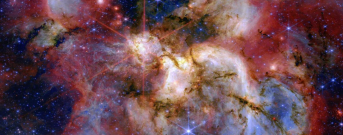
\includegraphics[width=0.55\textwidth]{img/w51_original_panel.png} % REEMPLAZAR: recorte del panel "Imagen Original" de la app
    \caption{Panel de imagen original en la herramienta, mostrando la región W51 tal como fue cargada, sin ningún procesamiento aplicado.}
    \label{fig:original_panel}
\end{figure}

\subsubsection{Análisis de histogramas originales}

Antes de aplicar cualquier transformación, la herramienta genera automáticamente los histogramas de los tres canales RGB de la imagen original para cada canal por separado. Estos histogramas muestran la distribución real de intensidades tal como aparece en la imagen base. El eje horizontal representa el valor de intensidad del píxel (de 0 a 255) y el eje vertical indica la cantidad de píxeles con ese valor.

\begin{figure}[H]
    \centering
    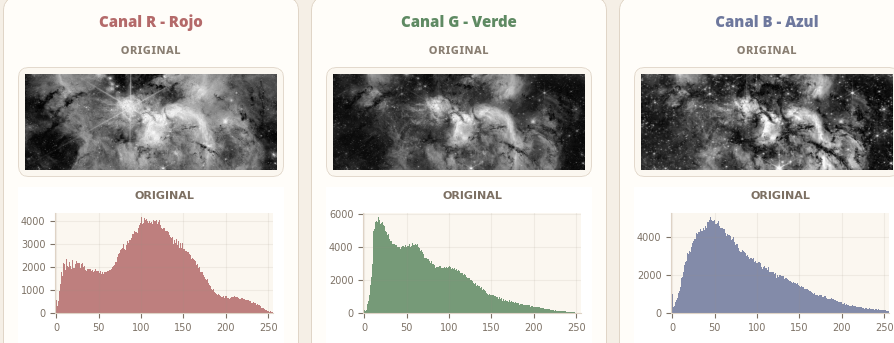
\includegraphics[width=0.92\textwidth]{img/histogramas_originales_rgb.png} % REEMPLAZAR: captura de las tres tarjetas de canal mostrando los histogramas "ORIGINAL"
    \caption{Histogramas originales de los canales R, G y B de la imagen W51, generados por la herramienta antes de aplicar ninguna transformación.}
    \label{fig:hist_orig}
\end{figure}

Los tres canales de la imagen infrarroja del JWST presentan distribuciones distintas. El canal rojo concentra sus valores en el rango de 0 a 250, con mayor densidad entre 50 y 180, correspondiente a la emisión general del gas caliente. El canal verde presenta su concentración entre 0 y 100, con una caída pronunciada a partir de los 50 niveles de intensidad, reflejando el contraste entre el polvo frío y el gas ionizado. El canal azul muestra una distribución similar al verde pero con la masa principal de píxeles concentrada entre 0 y 80, correspondiente a estructuras más frías o alejadas del frente de ionización.

\subsubsection{Normalización por canales}

La normalización por canal es una técnica de preprocesamiento que redistribuye los valores de intensidad dentro de un rango seleccionado manualmente, llevándolo a ocupar el espacio completo de 0 a 255. Su utilidad concreta consiste en que, si la información útil de un canal se concentra en un rango estrecho, al estirar ese rango se amplían las diferencias de brillo entre estructuras y se mejora el contraste visual \cite{gonzalez}.

La fórmula aplicada corresponde a la normalización min-max:
\begin{equation}
    p_{nuevo} = \frac{p - p_{\min}}{p_{\max} - p_{\min}} \times 255
    \label{eq:normalizacion}
\end{equation}
donde $p$ es el valor original del píxel, $p_{\min}$ y $p_{\max}$ son los límites inferior y superior del rango elegido, y $p_{nuevo}$ es el valor resultante. Los píxeles por debajo de $p_{\min}$ se fijan en 0 y los que superan $p_{\max}$ se fijan en 255. La implementación en \texttt{modelo.py} aplica esta fórmula de forma independiente sobre cada canal, procesando el arreglo NumPy completo sin iterar sobre píxeles individuales.

Los rangos aplicados a cada canal para la imagen W51 son los siguientes:

\textbf{Canal rojo: $p_{\min} = 36$, $p_{\max} = 170$.} El canal rojo presenta el rango más amplio entre los tres canales. Al excluir los 36 niveles inferiores (fondo oscuro del espacio) y recortar la saturación a partir de 170, se evita que las zonas de mayor brillo del gas ionizado dominen la normalización, preservando la información de contraste en las regiones intermedias donde se encuentran las estructuras estelares en formación.

\textbf{Canal verde: $p_{\min} = 88$, $p_{\max} = 255$.} El canal verde concentra su información útil a partir de los 88 niveles de intensidad. Al fijar el mínimo en ese punto, se eliminan los píxeles oscuros del fondo que no aportan información relevante y se expande el rango efectivo hacia el límite superior, logrando el mayor incremento de contraste en bordes y filamentos de polvo.

\textbf{Canal azul: $p_{\min} = 35$, $p_{\max} = 255$.} El canal azul presenta una distribución concentrada en valores bajos. Al establecer el mínimo en 35 se descartan únicamente los niveles más oscuros del fondo, y al mantener el máximo en 255 se aprovecha toda la información disponible en el canal, ampliando la representación de las estructuras más frías de la región.

Una vez normalizados los tres canales de forma independiente, se reconstruye la imagen RGB normalizada ($RGB_{norm}$) apilando los canales resultantes mediante \texttt{np.stack}. Esta imagen sirve como entrada única y coherente para los procesos de la segunda etapa.

\subsubsection{Histogramas normalizados}

Tras aplicar la normalización se generan automáticamente los histogramas correspondientes a cada canal, que la herramienta muestra en las tarjetas de canal (sección ``NORMALIZADO'') junto al histograma original, permitiendo una comparación directa.

\begin{figure}[H]
    \centering
    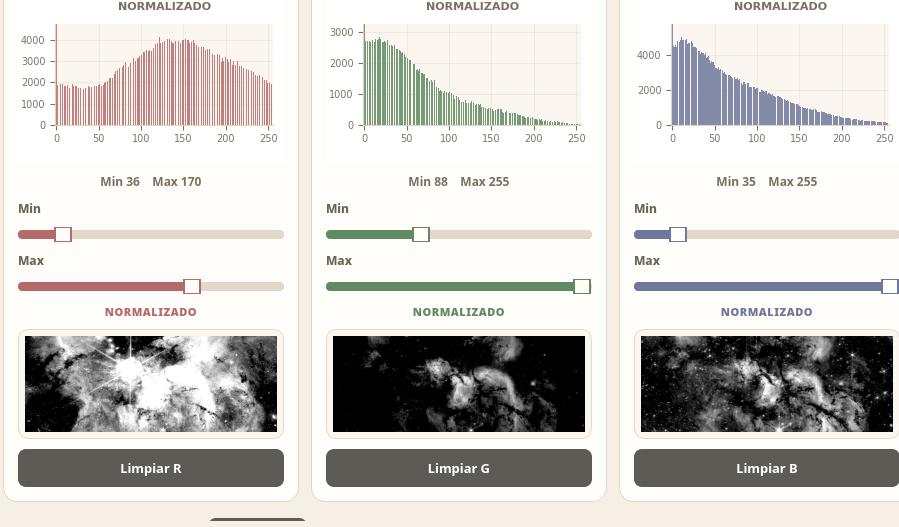
\includegraphics[width=0.92\textwidth]{img/histogramas_normalizados_rgb.png} % REEMPLAZAR: captura de las tres tarjetas mostrando los histogramas "NORMALIZADO"
    \caption{Histogramas normalizados de los canales R ($p_{\min}=36$, $p_{\max}=170$), G ($p_{\min}=88$, $p_{\max}=255$) y B ($p_{\min}=35$, $p_{\max}=255$) tras aplicar la expansión min-max.}
    \label{fig:hist_norm}
\end{figure}

En los tres canales se observa que la distribución se expande y ocupa un tramo más amplio del eje de intensidades respecto al histograma original. Los valores inferiores al $p_{\min}$ de cada canal se acumulan en el extremo izquierdo (valor 0) y los superiores al $p_{\max}$ en el extremo derecho (valor 255). La distribución intermedia, que en el original estaba comprimida, queda ahora repartida a lo largo del rango completo de 0 a 255. Esto se traduce en mayores diferencias de brillo entre píxeles vecinos, mecanismo por el cual la normalización mejora el contraste percibido de la imagen.

\subsubsection{Comparación entre imagen original y normalizada}

La comparación entre la imagen original y la imagen normalizada evidencia el efecto del procesamiento aplicado. La herramienta muestra ambas versiones en la pantalla de normalización: el panel ``Imagen Original'' y el panel ``Resultado Normalizado''.

\begin{figure}[H]
    \centering
    \begin{minipage}[t]{0.46\textwidth}
        \centering
        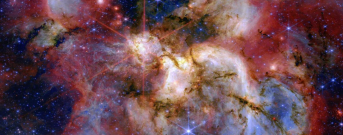
\includegraphics[width=\textwidth]{img/w51_original_panel.png} % REEMPLAZAR: recorte del panel "Imagen Original"
        \\[3pt]\small (a) Imagen original
    \end{minipage}
    \hfill
    \begin{minipage}[t]{0.46\textwidth}
        \centering
        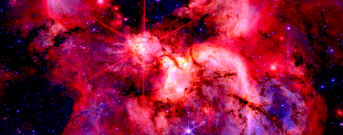
\includegraphics[width=\textwidth]{img/w51_normalizada_panel.png} % REEMPLAZAR: recorte del panel "Resultado Normalizado"
        \\[3pt]\small (b) Imagen normalizada
    \end{minipage}
    \caption{Comparación entre la imagen original de W51 y la imagen normalizada tras aplicar la expansión min-max con los rangos R[36--170], G[88--255], B[35--255].}
    \label{fig:comparacion_norm}
\end{figure}

Tras la normalización, la imagen presenta un contraste notablemente más amplio. Las zonas oscuras del original, que correspondían a regiones de polvo frío donde se encuentran estrellas en formación, comienzan a revelar estructuras antes indiferenciadas. El efecto más evidente se aprecia en los tonos rojos y violáceos que emergen en la imagen normalizada, producto de la expansión de los tres canales de forma independiente. La normalización no crea información nueva: redistribuye las intensidades para que la información ya presente resulte perceptible visualmente.

\subsubsection{Análisis de canales Rojo, Verde y Azul}

Una vez observada la mejora general de la imagen, la herramienta permite analizar cada canal de color de forma independiente. Para cada canal se muestra su versión original (en escala de grises representando únicamente ese canal) y su versión normalizada, junto con los sliders de rango \textit{min} y \textit{max} que permiten ajustar el rango de normalización de forma interactiva.

\begin{figure}[H]
    \centering
    \includegraphics[width=0.92\textwidth]{img/canales_rgb_tarjetas.png} % REEMPLAZAR: captura de las tres tarjetas (R, G, B) con sus vistas original, normalizada y sliders
    \caption{Tarjetas de análisis por canal de la herramienta. Cada tarjeta muestra la imagen del canal original (en grises), el histograma original y normalizado, los sliders de rango y la vista normalizada del canal.}
    \label{fig:canales_tarjetas}
\end{figure}

\textbf{Canal rojo ($p_{\min}=36$, $p_{\max}=170$).} Concentra la información sobre la emisión del gas caliente y la iluminación general de la región. Su histograma original es el más amplio de los tres. La normalización elimina el fondo oscuro (por debajo de 36) y recorta la saturación extrema (por encima de 170), expandiendo la información de contraste en los valores intermedios donde residen las estructuras estelares.

\textbf{Canal verde ($p_{\min}=88$, $p_{\max}=255$).} Presenta el mejor equilibrio entre zonas de polvo frío y gas ionizado. Al establecer el mínimo en 88 se eliminan los píxeles de fondo que no aportan información, y la expansión desde ese punto hasta 255 genera el mayor incremento de contraste local, haciendo visibles bordes, filamentos y estructuras intermedias que no se distinguen en el canal original.

\textbf{Canal azul ($p_{\min}=35$, $p_{\max}=255$).} Contiene información de estructuras más frías. Su histograma original está concentrado en valores bajos. Al recortar solo el fondo más oscuro (por debajo de 35) y mantener el máximo en 255, se aprovecha toda la información disponible. Este canal amplifica la representación de las zonas de menor temperatura en la región, aportando profundidad visual a la imagen normalizada final.

\subsubsection{Compresión, escala de grises y binarización}

Tras haber mejorado la visualización mediante la normalización, la segunda pantalla de la herramienta aplica tres transformaciones sucesivas sobre la imagen normalizada: conversión a escala de grises por ponderación de luminosidad, compresión espacial por promediado de bloques y binarización por umbral global \cite{jain}.

La conversión a escala de grises aplica la fórmula de luminosidad ponderada:
\begin{equation}
    I_{gris} = 0.299 \cdot R + 0.587 \cdot G + 0.114 \cdot B
    \label{eq:grises}
\end{equation}
Esta ponderación corresponde al modelo de luminosidad perceptual estándar (Rec.~601) \cite{gonzalez} y es la que implementa la función \texttt{gris\_luma} en \texttt{modelo.py}.

Sobre la imagen en escala de grises se aplica la compresión por bloques: cada región de $N \times N$ píxeles se reemplaza por su valor promedio, lo que reduce la resolución espacial de la imagen y actúa como filtro de suavizado que atenúa el ruido de alta frecuencia sin comprometer los bordes de mayor contraste \cite{szeliski}. La imagen ampliada se genera con \texttt{np.repeat} para mantener las dimensiones originales.

Finalmente, la binarización aplica un umbral global $T$ sobre la imagen comprimida: los píxeles con intensidad mayor o igual a $T$ se convierten en blanco (255) y el resto en negro (0).

\begin{figure}[H]
    \centering
    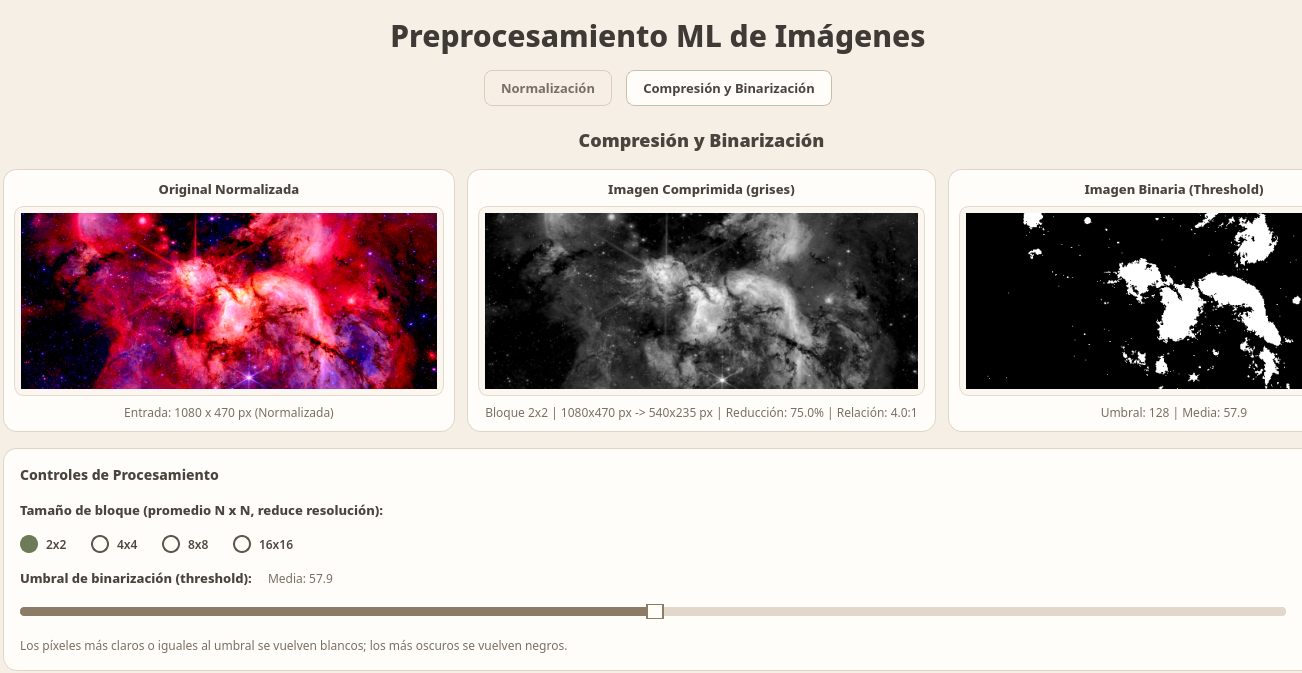
\includegraphics[width=0.92\textwidth]{img/compresion_binarizacion_pantalla.png} % REEMPLAZAR: captura de la pantalla "Compresión y Binarización" completa
    \caption{Segunda etapa del procesamiento en la herramienta: imagen normalizada de entrada (1080×470 px), imagen comprimida en escala de grises con bloque $2\times2$ (reducción del 75\%, relación 4.0:1) e imagen binaria con umbral $T=128$.}
    \label{fig:compresion_binaria}
\end{figure}

\subsubsection{Controles de procesamiento}

La herramienta expone dos controles interactivos que influyen directamente sobre el resultado:

\textbf{Tamaño de bloque.} Este control define el tamaño $N$ de la región cuadrada que se promedia en la compresión. Las opciones disponibles son $2 \times 2$, $4 \times 4$, $8 \times 8$ y $16 \times 16$. Su comportamiento es el siguiente:
\begin{itemize}
    \item \textbf{$2 \times 2$:} conserva la mayor parte del detalle fino. La simplificación es ligera y las estructuras de menor tamaño se mantienen visibles.
    \item \textbf{$4 \times 4$:} reduce más información y aplica una simplificación intermedia, difuminando gradualmente los detalles más pequeños.
    \item \textbf{$8 \times 8$:} simplifica la imagen en mayor medida; útil para observar patrones generales de brillo, pero los elementos pequeños pierden nitidez.
    \item \textbf{$16 \times 16$:} reduce agresivamente la información fina y puede ocultar estructuras de tamaño reducido, por lo que no es adecuado cuando se busca preservar detalles.
\end{itemize}

\textbf{Umbral de binarización.} Este control, implementado mediante un slider de 0 a 255, establece el valor límite que separa las regiones claras de las oscuras. Un umbral alto restringe la selección a las zonas más brillantes (gas ionizado, estrellas masivas), mientras que un umbral bajo amplía la selección incluyendo regiones de menor intensidad, con el riesgo de incorporar más ruido. La herramienta muestra en tiempo real el valor del umbral seleccionado y el valor de la media de la imagen comprimida como referencia para la selección del umbral.

\begin{figure}[H]
    \centering
    \begin{minipage}[t]{0.46\textwidth}
        \centering
        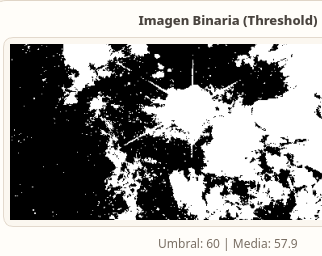
\includegraphics[width=\textwidth]{img/binaria_umbral_bajo.png} % REEMPLAZAR: imagen binaria con umbral bajo (ej. T=60 o T=84)
        \\[3pt]\small (a) Binarización con umbral bajo ($T \approx 60$)
    \end{minipage}
    \hfill
    \begin{minipage}[t]{0.46\textwidth}
        \centering
        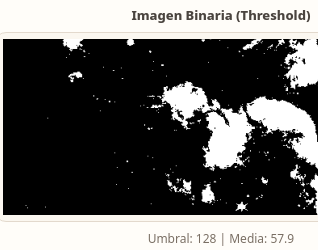
\includegraphics[width=\textwidth]{img/binaria_umbral_128.png} % REEMPLAZAR: imagen binaria con T=128 (valor usado en el informe)
        \\[3pt]\small (b) Binarización con umbral $T = 128$
    \end{minipage}
    \caption{Comparación del efecto del umbral de binarización sobre la imagen W51 comprimida (bloque $2\times2$, media = 57.9). Un umbral bajo clasifica como blanco más regiones, incorporando zonas de brillo medio; un umbral alto ($T=128 > $ media) restringe la selección a las zonas de mayor intensidad, principalmente el gas ionizado y las estrellas masivas.}
    \label{fig:comparacion_umbrales}
\end{figure}

\subsubsection{Resultados finales}

Como cierre del procesamiento, se presentan las tres imágenes que resumen el recorrido visual completo: la imagen original de W51, la imagen normalizada y la imagen comprimida en escala de grises. Esta comparación evidencia cómo estructuras poco perceptibles al inicio —estrellas en formación detrás de nubes de polvo— se vuelven visibles después del procesamiento.

\begin{figure}[H]
    \centering
    \begin{minipage}[t]{0.31\textwidth}
        \centering
        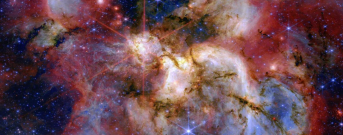
\includegraphics[width=\textwidth]{img/w51_original_panel.png} % REEMPLAZAR: imagen original de W51
        \\[3pt]\small (a) Imagen original
    \end{minipage}
    \hfill
    \begin{minipage}[t]{0.31\textwidth}
        \centering
        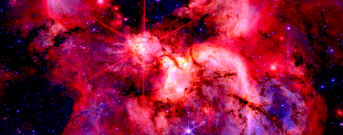
\includegraphics[width=\textwidth]{img/w51_normalizada_panel.png} % REEMPLAZAR: imagen normalizada R[36-170] G[88-255] B[35-255]
        \\[3pt]\small (b) Imagen normalizada
    \end{minipage}
    \hfill
    \begin{minipage}[t]{0.31\textwidth}
        \centering
        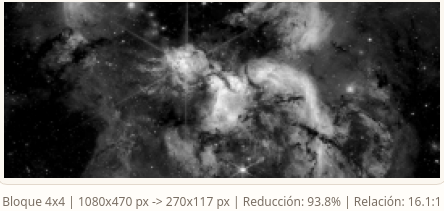
\includegraphics[width=\textwidth]{img/w51_gris_comprimida.png} % REEMPLAZAR: imagen en escala de grises con bloque 2x2
        \\[3pt]\small (c) Imagen comprimida en grises
    \end{minipage}
    \caption{Comparación final del flujo de procesamiento sobre la imagen W51: imagen original (sin procesar), imagen normalizada con expansión min-max por canal, e imagen comprimida en escala de grises con bloque $2\times2$.}
    \label{fig:resultados_finales}
\end{figure}

\subsection{Habilidades blandas empleadas en la práctica}
$\blacksquare$ Trabajo en equipo \\
$\blacksquare$ Responsabilidad \\
$\blacksquare$ Pensamiento crítico

\subsection{Conclusiones}
\begin{enumerate}
    \item La normalización min-max por canal resultó ser la técnica más efectiva para maximizar el rango dinámico de la imagen de la región W51, redistribuyendo las intensidades de cada canal de forma independiente y permitiendo revelar estructuras estelares que en la imagen original aparecían ocultas detrás de las nubes de gas.

    \item El análisis por canales RGB evidenció que cada canal aporta información espectral diferente sobre la región: el canal rojo concentra la emisión general del gas caliente, el canal verde ofrece el mejor contraste entre el polvo frío y el gas ionizado, y el canal azul presenta la distribución más estrecha, correspondiente a estructuras más frías.

    \item La implementación de una arquitectura modular (MVVM) permitió separar la lógica matemática de transformación de imagen (\texttt{modelo.py}) del manejo de eventos y el estado de la interfaz, garantizando que las transformaciones sean puras y deterministas, y que el flujo de normalización $\to$ conversión a grises $\to$ compresión $\to$ binarización se ejecute de forma coherente ante cualquier cambio de parámetro.
\end{enumerate}

\subsection{Recomendaciones}
\begin{enumerate}
    \item Utilizar imágenes con histogramas bien definidos y de buena resolución, ya que la calidad de la imagen de entrada influye directamente en la claridad de los resultados tras la normalización, la compresión y la binarización.

    \item Ajustar de forma cuidadosa los rangos mínimo y máximo de cada canal, así como el tamaño de bloque y el umbral de binarización, teniendo en cuenta que valores inadecuados pueden eliminar detalles relevantes o introducir ruido en el resultado final.

    \item Se sugiere integrar en futuras versiones un algoritmo de umbralización adaptativa (como el método de Otsu \cite{opencv_doc}) para automatizar la selección del umbral de binarización en imágenes con iluminación no uniforme, reduciendo la dependencia del ajuste manual.
\end{enumerate}

\subsection{Referencias bibliográficas}
{
    \renewcommand{\refname}{}
    \vspace{-1.5em}

    \begin{thebibliography}{99}
        \bibitem{gonzalez}
        R. C. Gonzalez and R. E. Woods, \textit{Digital Image Processing}, 4th ed. New York, NY, USA: Pearson, 2018.

        \bibitem{jain}
        A. K. Jain, \textit{Fundamentals of Digital Image Processing}. Englewood Cliffs, NJ, USA: Prentice Hall, 1989.

        \bibitem{szeliski}
        R. Szeliski, \textit{Computer Vision: Algorithms and Applications}, 2nd ed. Cham, Switzerland: Springer, 2022.

        \bibitem{opencv_doc}
        OpenCV Team, ``Image Thresholding,'' in \textit{OpenCV Documentation}, version 4.x. [Online]. Available: \texttt{https://docs.opencv.org/4.x/d7/d4d/tutorial\_py\_thresholding.html}

        \bibitem{jwst_w51}
        H.~Yoo and A.~Ginsburg, ``Star formation in W51: First JWST observations,'' University of Florida, Gainesville, FL, USA, 2025. Crédito de imagen: NASA, ESA, CSA, Yoo \& Ginsburg (UF); Procesamiento: A.~Pagan (STScI). [Online]. Available: \texttt{https://www.nasa.gov/missions/webb/}
    \end{thebibliography}
}

\end{document}
